%!TEX ROOT = thesis.tex
\chapter{INTRODUCTION}
\section{Introduction to Semantic Segmentation}

The last few years have seen a massive surge in research regarding deep learning applications in computer vision with the most common one being object detection, where a network accept an image as an input and output either a single or multi class label. Typically, the position of detected objects are defined by rectangular coordinates that are represented by bounding boxes. However, in a lot of image processing task, such as in satellite images analysis the target output should include more accurate localization. The bounding box may have more than one objects inside it. To increase its localization, instead of assigning a set of labels to an image, semantic segmentation would label each pixel independently. After each pixel is labelled, a new image, called the mask  will be produced with every pixels being coloured according to its label.

The emergence of the term "semantic segmentation" can be traced back to the 1970s \cite{YU201882}. At that time, this terminology was equivalent to non-semantic image segmentation but emphasized that the segmented regions must contain a "semantic meaning" hence where the semantic part of the word comes from. Semantic segmentation algorithms calssify each pixel into a class. On the other hand, non-semantic segmentation algorithms try to detect consistent regions or region boundaries and it can be solved using many unsupervised algorithms. 

In the 1990s, “object segmentation and recognition” is a two-class image segmentation problem which is to separate foreground objects from background. As the task is quite challenging, a relaxed two-class image segmentation problem: the sliding window object detection, was proposed to partition objects with bounding boxes. However, two-class image segmentation cannot tell what these segmented objects are. As a result, the generic sense of object detection was gradually extended to multi-class image labeling, which is the present definition of semantic segmentation, to tell both where and what the objects in the scene.

\begin{figure}[ht]
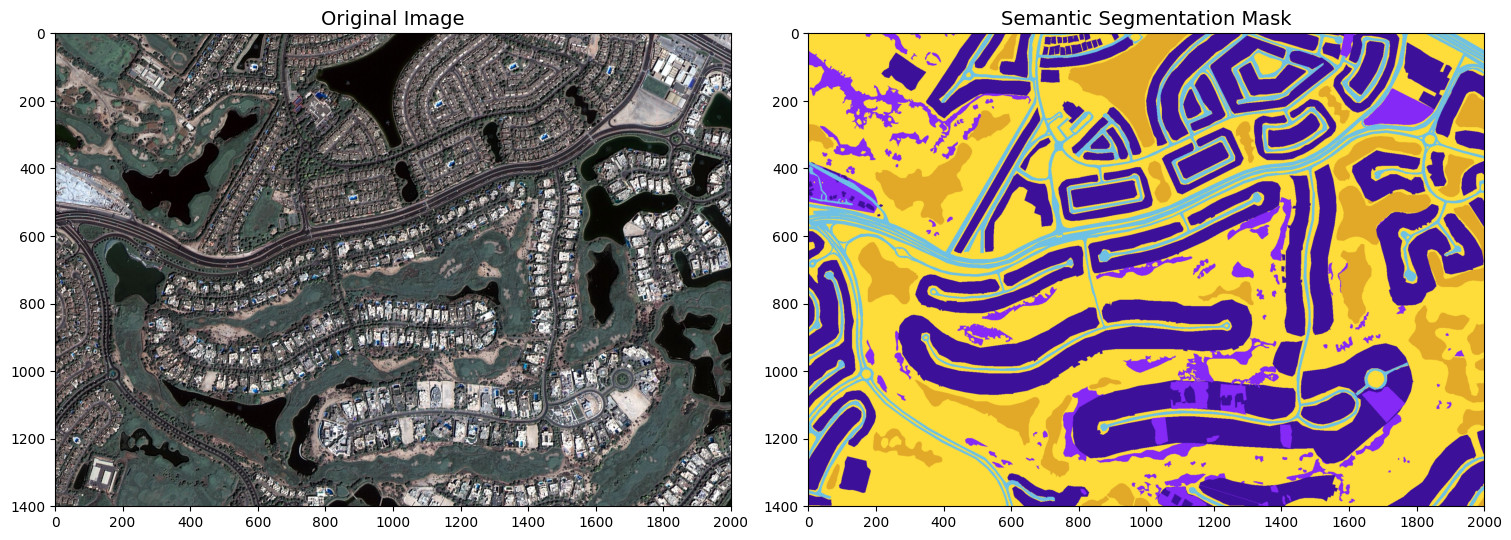
\includegraphics[width=12cm, height=6cm]{images/semantic segmentation example.jpg}
\centering
\caption{Semantic Segmentation of a Satellite Image}
\label{fig:example of semantic segmentation}
\end{figure}

\begin{figure}[ht]
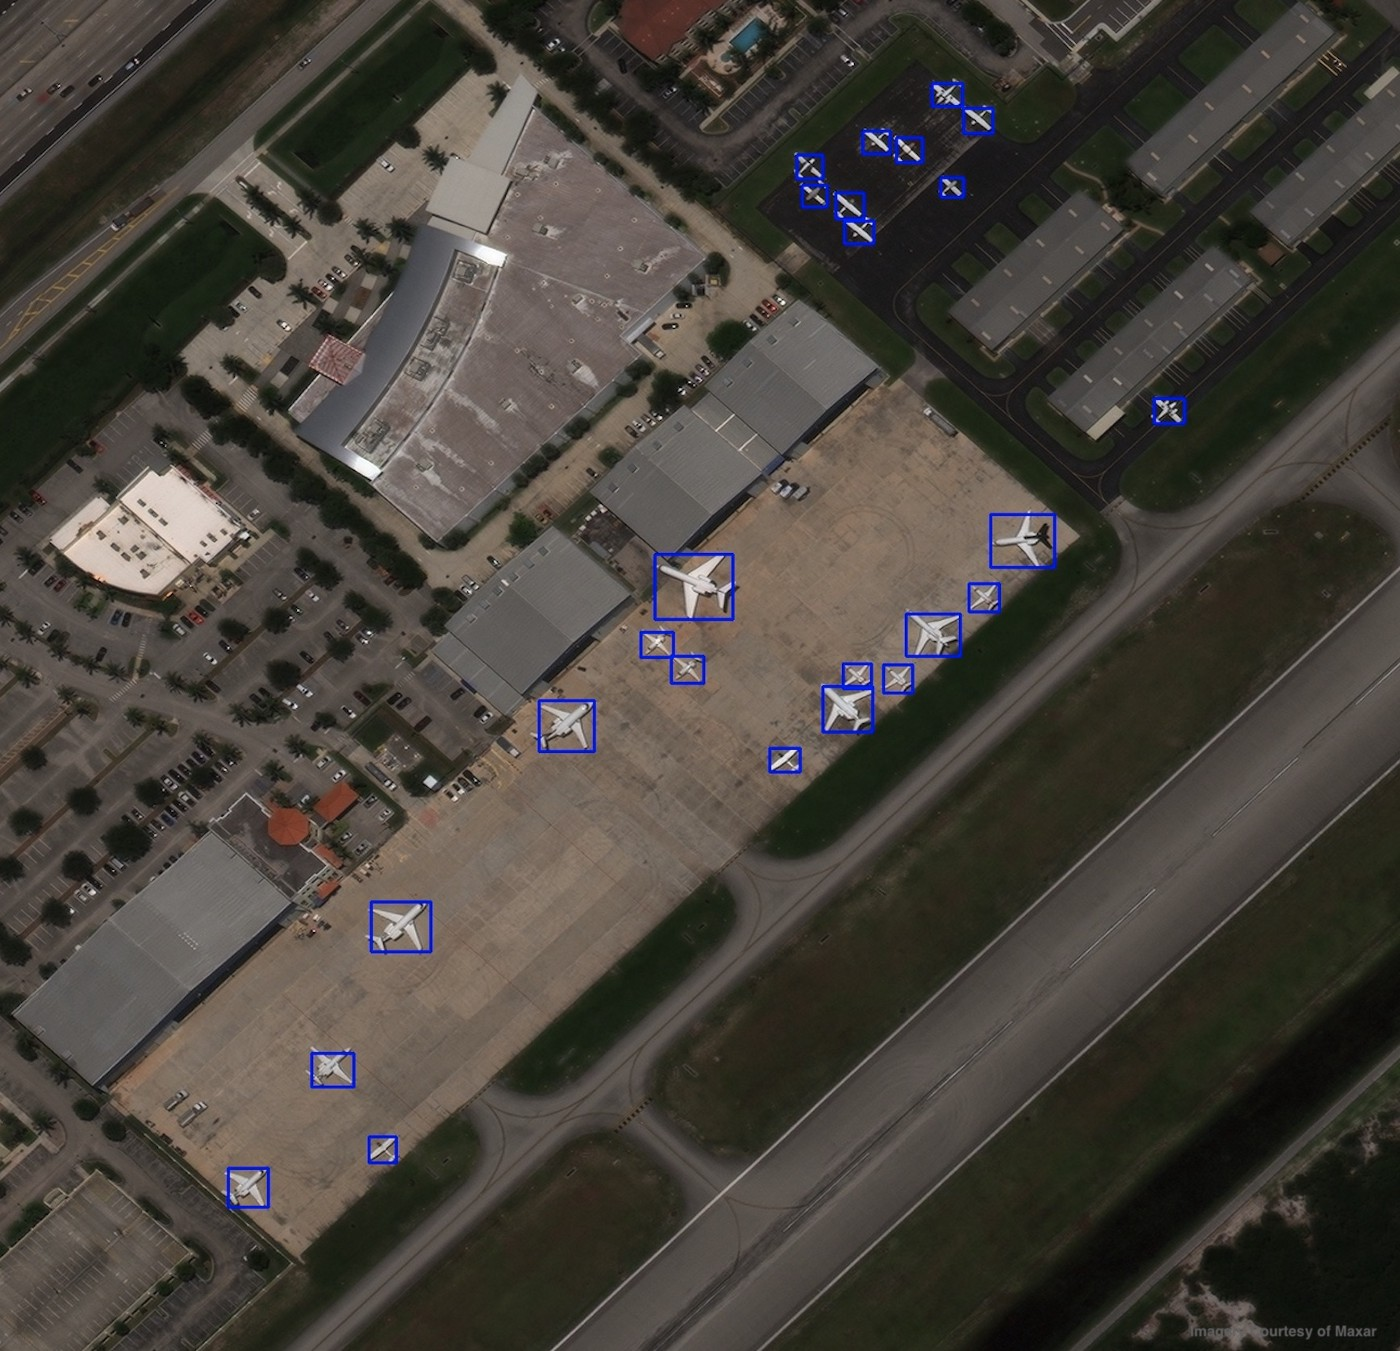
\includegraphics[width=9cm, height=5cm]{images/airport object detection.jpeg}
\centering
\caption{Object Detection of a Satellite Image}
\label{fig:airport object detection}
\end{figure}

\section{Introduction to Satellite Images}

Satellite images are images of the Earth that are collected by observation satellites. Observation satellites are satellites that are designed to observe the Earth from orbit while equipped with sensors that measure a range of  electromagnetic spectrum such as UV, visible, infrared, microwave, or radio. 

There are 3 types of resolution that one should consider when working with satellite images. Namely the resolutions are the spatial resolution, spectral resolution and temporal resolution.

Spatial resolution refers to the smallest feature that is displayed by an image. In most datasets it is usually represented as a single numerical value representing one side of a square pixel. For example, a spatial resolution of 10m means that a single pixel represents an area of 10 m\textsuperscript{2}.

Spectral resolution refers to the extent of the sensors on the satellite to detect and measure wavelengths on the electromagnetic spectrum. The finer the spectral resolution, the narrower the wavelength range for a particular channel or band. Images with high spectral resolution is important in computer vision because  classes such as rock types and soil types would require an analysis at a much finer spectrum to distinguish them.

\FloatBarrier
\begin{table}[!h]
\centering
\begin{tabular}{|l|l|l|}
\hline
\textbf{Spectral Bands} & \textbf{Wavelength }$\mu \textbf{m}$ & \textbf{Description}                                                                                                                                                     \\ \hline
Band 1                  & 400 - 450           & \begin{tabular}[c]{@{}l@{}}Least absorbed by water, and will be very\\ useful in bathymetric studies.\end{tabular}                                                       \\ \hline
Band 2                  & 450 -510            & Provides good penetration of water.                                                                                                                                      \\ \hline
Band 3                  & 510 - 580           & Ideal for calculating plant vigor.                                                                                                                                       \\ \hline
Band 4                  & 585 - 625           & \begin{tabular}[c]{@{}l@{}}Detects the “yellowness” of particular\\ vegetation.\end{tabular}                                                                             \\ \hline
Band 5                  & 630 - 690           & \begin{tabular}[c]{@{}l@{}}Better focused on the absorption of\\ red light.\end{tabular}                                                                                 \\ \hline
Band 6                  & 705 - 745           & \begin{tabular}[c]{@{}l@{}}Centered strategically at the onset of\\ the high reflectivity portion of vegetation\\ response\end{tabular}                                  \\ \hline
Band 7                  & 770 - 895           & \begin{tabular}[c]{@{}l@{}}Effectively separates water bodies from\\ vegetation, identifies types of vegetation\\ and also discriminates between soil types\end{tabular} \\ \hline
Band 8                  & 860 - 1040          & \begin{tabular}[c]{@{}l@{}}Overlaps Band 7 but is less\\ affected by atmospheric influence.\end{tabular}                                                                 \\ \hline
\end{tabular}
\caption{Different purposes of spectral bands of satellite images}
\label{tab:spectral_bands}
\end{table}
\FloatBarrier

Lastly, temporal resolution refers to the time period between capturing two consecutive images of the same surface area. In some literature it is also called the satellite revisit period. An image with a higher temporal resolution has a lower time period between two consecutive images. For example an image with a temporal resolution of two days means that a satellite will capture an image of the same area every two days.  For some satellites, a constellation of satellites are used to increase temporal resolution. As an example the SENTINEL-2 mission actually use 2 satellites with each having a revisit period of 10 days making the temporal resolution to be effectively 5 days. Temporal resolutions are important to detect changes that occur during a specified time period.

\section{Applications of Semantic Segmentation of Satellite Images}

\begin{enumerate}
    \item \textbf{Land Cover Mapping}
    
    Land cover mapping is the process of constructing a cover map that provide information about the Earth's surface cover pattern and land use. Such example of information provided are vegetation index and soil index. Covers maps are important for agricultural monitoring, public policy development and urban planning. Land cover mapping utilizes semantic segmentation of satellite images. Before the advances of deep learning, land cover mapping relies on traditional semantic segmentation techniques such Support Vector Machines and Random Decision Forest \cite{DBLP:journals/corr/Thoma16a}. However, semantic segmentation requires a huge number of features to distinguish huge variations of land patterns. Traditional methods that only rely on low-level spectral and spatial resolution have been proven to be less optimal than its  deep learning alternative due to the latter's ability to extract multilevel and multi-scale features\cite{Yuan2020DeepLI}. 
    
    \item \textbf{Water Bodies Detection}

    Semantic segmentation of satellite images has long been used in detecting bodies of water such as lakes and natural springs in areas where water is a scarce resource. One of the most popular traditional technique is normalized difference water index (NDWI). This technique heavily relies on IR band and measure the reflectance characteristics of water. This technique is very susceptive to noise and quite complex to develop and deploy. However, deep learning has been proven to be more reliable than NDWI, a CNN based network reached an accuracy of 99.86\% \cite{edseee.864274320181101}.
    
    \item \textbf{Soil Erosion Detection}
    
    Understanding soil attributes is an important step for the construction industry. As most construction projects require excavation ((e.g.,piping, laying foundation, tunneling), soil attributes could affect the entire excavation process concerning scheduling, resource planning, procurement, claim resolution, and safety considerations. Soil classification is a process of categorizing soil based on similar attributes. The traditional involves on-site sampling and analysing the samples in a laboratory which is very time consuming and expensive. Thanks to deep learning ability to utilizes high resolution images, a CNN based network was developed to classify soil based on semantic segmentation of satellite images \cite{9554290}. 
    
    \item \textbf{Flood Detection and Assessment System}
    
    Due to climate change, flooding has quickly becoming one of the most destructive and frequent type of natural disaster, and this trend is expected to continue. Detecting flood prior of its occurrence has been vital to save lives and minimizes financial loss. On top of that, a lot of agencies around the world require a system to assess the total  destruction from flooding. The assessment method is usually done manually using aerial images. Semantic segmentation has been widely used as a tool to aid in the process of designing and deploying accurate flood detection and post-flood assessment system \cite{edseee.988427220220717}. 
\end{enumerate}

\section{Problem Statement}

\begin{enumerate}
    \item Most of the models reviewed are either not trained using satellite images or the dataset have very low resolution and dimensions. 
    \item Most of the semantic segmentation models reviewed are proposed before 2022 and they use CNN as Vision Transformer is a new development.  
    \item Vision Transformer models are too large hence making it unsuitable for real-world applications.
    \end{enumerate}


\section{Project Objectives}
\begin{enumerate}
    \item Identify suitable datasets of satellite images that will be used for training and validation. Multiple datasets will be evaluated and a new dataset would be constructed if necessary. The dataset must contain a minimal class imbalanced.
    \item Identify and train a semantic segmentation model with a Transformer-based encoder-decoder model to perform using chosen dataset to get a baseline result. We would also train a CNN model using the same dataset to get a comparison.
    \item Identify the appropriate steps that can be taken to compress the Transformer model while maintaining its performance.
\end{enumerate}
\section{Project Scope}

The scope of the dataset used in this project will be limited to satellite images. The chosen dataset must have a spatial resolution that is small enough to avoid any losses of information. On top of that, the dataset must be bigger than 240x240 pixels. The dataset must have been taken by a satellite. There is no restriction on the type of bands that the dataset can have.

The scope of the network proposed in this project must be one based on Vision Transformer.  The Vision Transformer network must be able to perform semantic segmentation task of satellite images. The performance of the proposed vision transformer network shall be compared to the  previous works trained on the same dataset.

\section{Chapter Organization}

This report is organized into 6 chapters. Chapter 1 would provide a brief introduction to satellite images and semantic segmentation, the applications of semantic segmentation of satellite images and the problems that this project aims to solve. Chapter 2 review the current literature that aims have similiar objectives to this project. It also contain a brief introduction to the semantic segmentation techniques before the advance of deep learning. Chapter 3 explains the fundamental theories to be understood before designing and implementing the model. Chapter 4 presents
the details of the project pipelines with clear distinctions of work to be done. Chapter 5
shows the implementation plan for both FYP1 and FYP2 including milestones as well
as preliminary results of experiments. Lastly, Chapter 6 provides a summary of work
done in FYP1 with findings, future directions, and problems encountered.
